\documentclass[]{beamer}
\usepackage[T1]{fontenc}
\usepackage[utf8]{inputenc}
\usepackage{lmodern}
\usepackage[italian]{babel}
\usepackage{mathrsfs}
\usepackage{cancel}

\title{Relatività}
\author{\texorpdfstring{Mattia Cozzi\newline\href{mailto:cozzimattia@gmail.com}{\texttt{cozzimattia@gmail.com}}}{Mattia Cozzi}}
\date{a.s.~2023/2024}

%\documentclass[handout]{beamer}     %usare questa classe per generare l'handout
%\usepackage{pgfpages}   %per mostrare più quadri nella stessa pagina
%\pgfpagesuselayout{4 on 1}[a4paper,border shrink=5mm,landscape]
\usetheme{Singapore}
%\useoutertheme[left]{sidebar} %elementi intorno alle diapositive
\setbeamercovered{dynamic} %modifica l'aspetto del testo grigetto delle diapositive future. Argomenti: invisible/transparent/dynamic
\usecolortheme{orchid}
%COLORE PRINCIPALE
\definecolor{marroncino}{RGB}{156, 26, 0} % UBC Blue (primary)
\setbeamercolor{structure}{fg=marroncino} % itemize, enumerate, etc

\theoremstyle{plain}
\newtheorem{teorema}{Teorema}

\usepackage{tikz}
\usepackage{circuitikz}


\usepackage{pgf,pgfplots,graphicx}
\usetikzlibrary{angles,quotes,arrows,shapes,decorations.markings}
\pgfplotsset{compat=1.15}
\usepgfplotslibrary{units,fillbetween} % to add units easily to axis
\tikzset{fleche/.style args={#1:#2}{postaction=decorate,decoration={name=markings,mark=at position #1 with {\arrow[#2,scale=2]{>}}},},}


\def\angolo[#1](#2)(#3:#4:#5)% Syntax: [draw options] (center) (initial angle:final angle:radius)
    { \draw[#1] ($(#2)+({#5*cos(#3)},{#5*sin(#3)})$) arc (#3:#4:#5); }

\begin{document}

\begin{frame}
  \titlepage
\end{frame}





\begin{frame}
\frametitle{Contenuti}
\tableofcontents
\end{frame}

%slide sull'invarianza della velocità della luce

\section{Luce}



\begin{frame}
\frametitle{Contesto storico}
\begin{columns}
\begin{column}{0.2\textwidth}
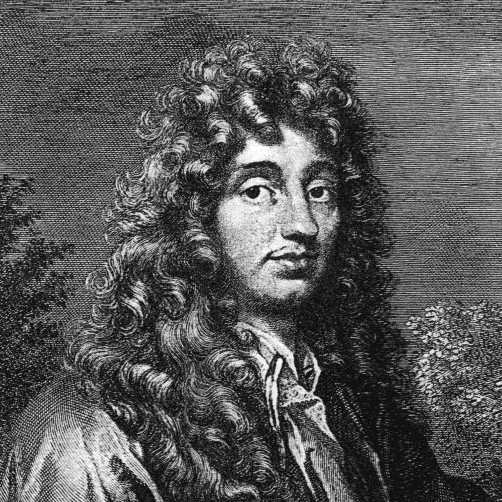
\includegraphics[width=\columnwidth]{img/huygens.jpg}

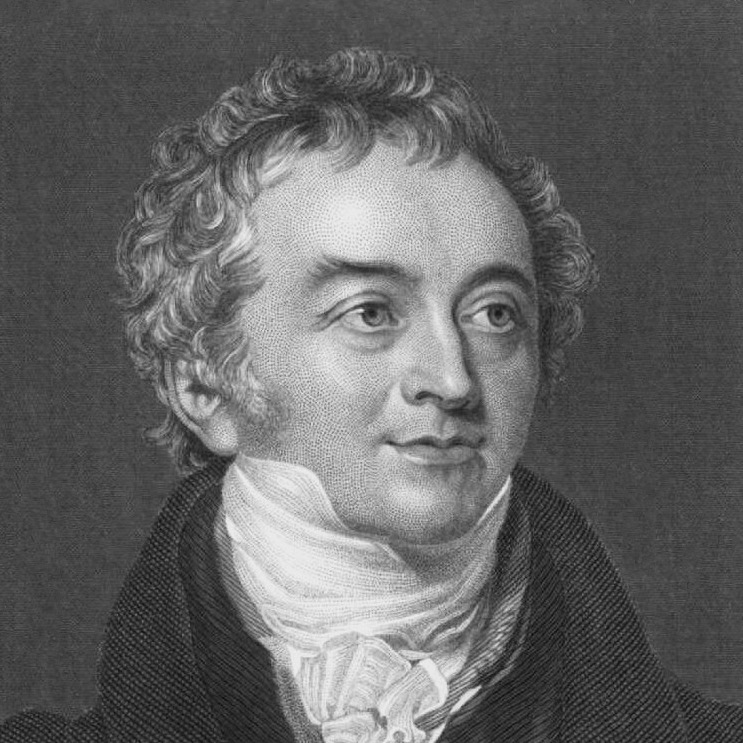
\includegraphics[width=\columnwidth]{img/young.jpg}

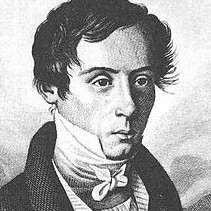
\includegraphics[width=\columnwidth]{img/fresnel.jpg}
\end{column}
\begin{column}{0.7\textwidth}
Nel 1678 \alert<1>{Huygens} formula una \emph{teoria ondulatoria della luce}, estesa poi da \alert<1>{Young} e \alert<1>{Fresnel} nel XIX secolo.\pause

\begin{small}
\begin{itemize}
\item<2-> la luce è intesa come un'onda che si propaga in un mezzo (l'\alert<2>{etere luminifero}, Young 1804) formato da particelle elastiche e che permea tutto l'universo;
\item<3-> nel XIX secolo la teoria di Huygens, grazie agli esperimenti su \alert<3>{interferenza} e \alert<3>{diffrazione}, è preferita a quella corpuscolare (Descartes 1637 e Newton 1672).
\end{itemize}
\end{small}
\end{column}
\end{columns}
\end{frame}



\begin{frame}
  \frametitle{Onde elettromagnetiche}
  Le onde elettromagnetiche:
  \begin{itemize}
    \item furono previste da Maxwell nel 1861 a partire dalle sue equazioni differenziali e dimostrate sperimentalmente da Heinrich Rudolph Hertz nel 1889;\pause
    \item non richiedono un mezzo materiale e si propagano anche nel vuoto;\pause
    \item si muovono nel vuoto a velocità:
    \begin{center}
    $ c = \dfrac{1}{\sqrt{\varepsilon_0 \mu_0}} = 2,998 \times 10^8 \, \frac{m}{s} $
    \end{center}
    e hanno come caso particolare la luce.
  \end{itemize}
\end{frame}



\section{Einstein}

\begin{frame}
\frametitle{Contesto}
\begin{columns}
\begin{column}{0.2\textwidth}
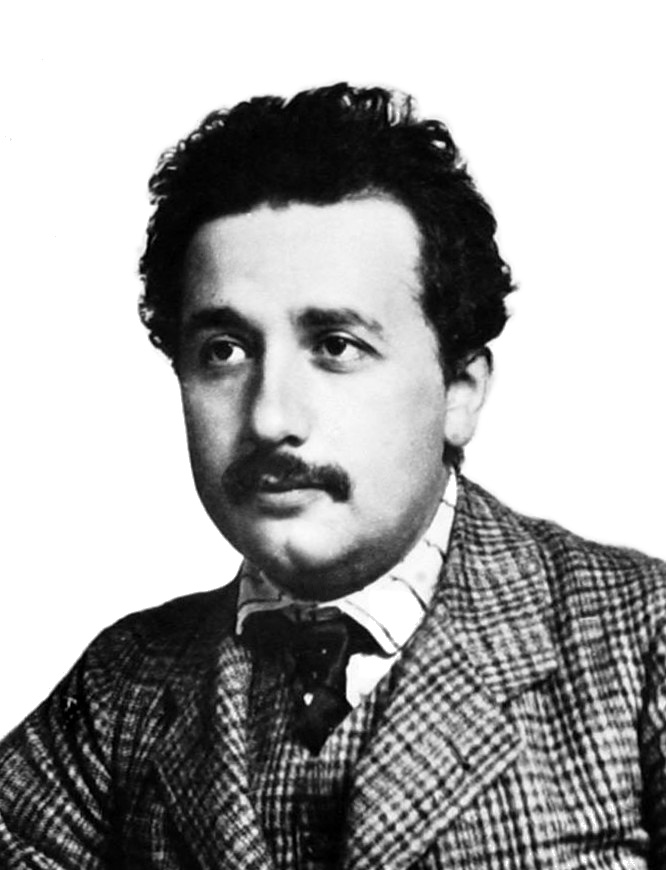
\includegraphics[width=\columnwidth]{img/einstein.jpg}
\end{column}
\begin{column}{0.7\textwidth}
\begin{center}
  1905
\end{center}
\emph{Annus mirabilis} di Einstein, che pubblica quattro articoli fondamentali.\pause

\begin{small}
\begin{enumerate}
\item<2-> studia l'effetto fotoelettrico, ipotizzando la \alert<2>{doppia natura della luce};
\item<3-> analizza il moto browniano, contribuendo ad affermare l'\alert<3>{ipotesi atomica della materia};
\item<4-> propone la \alert<4>{relatività ristretta} pur senza conoscere il risultato di M\&M, ma spinto da ragioni di semplicità ed eleganza formale;
\item<5-> dimostra l'equivalenza tra massa ed energia: \alert<5>{$ E=mc^2 $}.
\end{enumerate}
\end{small}
\end{column}
\end{columns}
\end{frame}





\begin{frame}
\frametitle{Assiomi della relatività ristretta}
La contraddizione restava aperta e fu affrontata da Einstein proponendo una rifondazione della fisica sulla base di \alert<1>{due assiomi}:\pause
\begin{block}{Principio di relatività ristretta\footnote{Estensione del principio di relatività galileiana, che vale solo per la meccanica.}}
  Le leggi e i principi della fisica hanno la stessa forma in tutti i sistemi di riferimento inerziali.
\end{block}\pause
\begin{block}{Principio di invarianza di $ c $}
La velocità della luce è la stessa in tutti i sistemi di riferimento inerziali, indipendentemente dal moto del sistema stesso o della sorgente da cui la luce è emessa.
\end{block}
\end{frame}



\begin{frame}
  \frametitle{Tempo assoluto?}
  Per giustificare l'invarianza di $ c $ Einstein parte dalla messa in discussione di un fatto che fino ad allora era stato dato per scontato: che il tempo scorresse \alert<1>{identico in ogni sistema di riferimento}, un tempo assoluto.\pause
  
  ~
  
  L'idea di fondo è che un fenomeno possa avere durate temporali diverse a seconda del sistema di riferimento dal quale viene effettuata la misurazione.\pause
  
  ~
  
  Introduciamo l'idea di \alert{durata propria di un fenomeno}, cioè la durata temporale del fenomeno quando la misurazione avviene da un sistema di riferimento in cui il fenomeno è fermo.\\
  La indicheremo con $ \Delta t $.
\end{frame}





\section{Fenomeni relativistici}




\begin{frame}
  \frametitle{Dilatazione dei tempi}
\begin{small}
    \begin{center}
\colorbox{marroncino!30}{$ \Delta t' = \dfrac{1}{\sqrt{1- \left( \dfrac{v}{c} \right)^2 }}\Delta t $}
  \end{center}
  \end{small}
  Essendo $ v \leq c $, il denominatore della formula precedente è sempre minore o uguale a 1, e pertanto $ \Delta t' \geq \Delta t $.\\~\pause
  \begin{block}{Dilatazione di tempi}
    La durata di un fenomeno è minima quando essa è misurata in un SDR solidale con il baricentro del sistema fisico in esame\footnote{Da qui il ``paradosso dei gemelli''.}.
  \end{block}
\end{frame}


\begin{frame}
  \frametitle{$ \beta $ e $ \gamma $}
  Definiamo \colorbox{marroncino!30}{$ \beta = \dfrac{v}{c} $} ($ \beta \leq 1 $){\pause} e pertanto:
\begin{center}
  \colorbox{marroncino!30}{$ \gamma = \dfrac{1}{\sqrt{1- \left( \frac{v}{c} \right)^2 }} = \dfrac{1}{\sqrt{1 - \beta^2}} $}
\end{center}
{\pause}e scriveremo semplicemente:
  \begin{center}
  \colorbox{marroncino!30}{$ \Delta t' = \gamma\Delta t $}
  \end{center}
  $ \gamma $ è detto \alert{fattore di Lorentz}.
\end{frame}


\begin{frame}
  \frametitle{Il fattore di Lorentz (1)}
  Possiamo leggere nel fattore $ \beta = \dfrac{v}{c} $ la percentuale della velocità della luce alla quale avviene il moto nel SDR considerato.{\pause}\\~\\  
  Ad esempio, se $ v = 1 \times 10^8 \, \frac{m}{s} $:
  \begin{center}
  $ \beta = \dfrac{1 \times 10^8 \, \frac{m}{s}}{3 \times 10^8 \, \frac{m}{s}} = \dfrac{1}{3} = 0,\overline{3} \approx 33 \% $
  \end{center}
  {\pause}
  Studiamo l'andamento di $ \gamma $ al variare di $ v $.
\end{frame}




\begin{frame}
  \frametitle{Il fattore di Lorentz (2)}
  
  
  \begin{columns}
\begin{column}{0.4\textwidth}

\scriptsize 
    \centering
  \begin{tabular}{c|c|c}
    $ \mathbf{\beta} $ & $ \mathbf{\gamma} $ & $ \mathbf{\gamma}^{-1} $\\\hline\rule{0pt}{3ex}
    $ 0,010 $ & $ 1,000 $ & $ 1,000 $ \\\rule{0pt}{3ex}
    $ 0,100 $ & $ 1,005 $ & $ 0,995 $ \\\rule{0pt}{3ex}
    $ 0,200 $ & $ 1,021 $ & $ 0,980 $ \\\rule{0pt}{3ex}
    $ 0,300 $ & $ 1,048 $ & $ 0,954 $ \\\rule{0pt}{3ex}
    $ 0,400 $ & $ 1,091 $ & $ 0,917 $ \\\rule{0pt}{3ex}
    $ 0,500 $ & $ 1,155 $ & $ 0,866 $ \\\rule{0pt}{3ex}
    $ 0,600 $ & $ 1,250 $ & $ 0,800 $ \\\rule{0pt}{3ex}
    $ 0,700 $ & $ 1,400 $ & $ 0,714 $ \\\rule{0pt}{3ex}
    $ 0,800 $ & $ 1,667 $ & $ 0,600 $ \\\rule{0pt}{3ex}
    $ 0,866 $ & $ 2,000 $ & $ 0,500 $ \\\rule{0pt}{3ex}
    $ 0,900 $ & $ 2,294 $ & $ 0,436 $ \\\rule{0pt}{3ex}
    $ 0,990 $ & $ 7,089 $ & $ 0,141 $ \\\rule{0pt}{3ex}
    $ 0,999 $ & $ 22,366 $ & $ 0,045 $ \\
  \end{tabular}

\end{column}
\begin{column}{0.6\textwidth}
\begin{figure}
\begin{tikzpicture}[xscale=1.4,yscale=.4]
\draw [->] (-.15,0) -- (3.5,0);
\draw [->] (0,-.5) -- (0,9);
\draw [dotted] (0.5,0) -- (0.5,1);
\draw [dotted] (1,0) -- (1,1.1);
\draw [dotted] (1.5,0) -- (1.5,1.2);
\draw [dotted] (2,0) -- (2,1.4);
\draw [dotted] (2.5,0) -- (2.5,1.8);
\draw [dotted] (3,0) -- (3,7.8);
\draw[smooth, orange, thick, domain=0:2.99, samples=50] plot 
({\x},{    (1- (.11*\x^2))^-.5           });
\node [below] at (.5,0) {{\tiny $ 0,5 $}};
\node [below] at (1,0) {{\tiny $ 1 $}};
\node [below] at (1.5,0) {{\tiny $ 1,5 $}};
\node [below] at (2,0) {{\tiny $ 2 $}};
\node [below] at (2.5,0) {{\tiny $ 2,5 $}};
\node [below] at (3,0) {{\tiny $ 3 $}};
\node [below] at (1.5,-1.5) {{\tiny $ v \, (\times 10^8 \, \frac{m}{s}) $}};
\node [left] at (0,1) {{\tiny $ 1 $}};
\node [left] at (0,2) {{\tiny $ 2 $}};
\node [left] at (0,3) {{\tiny $ 3 $}};
\node [left] at (0,4) {{\tiny $ 4 $}};
\node [left] at (0,5) {{\tiny $ 5 $}};
\node [left] at (0,6) {{\tiny $ 6 $}};
\node [left] at (0,7) {{\tiny $ 7 $}};
\node [left] at (0,8) {{\tiny $ 8 $}};
\node [left] at (-.3,4.5) {{\tiny $ \gamma $}};
\end{tikzpicture}

~

\footnotesize
$ \displaystyle \lim_{v \to c} \frac{1}{\sqrt{1- \left( \frac{v}{c} \right)^2 }} = + \infty  $


\end{figure}
\end{column}
\end{columns}
\end{frame}





\begin{frame}
  \frametitle{Contrazione delle lunghezze}
Oltre all'idea di tempo assoluto, dobbiamo anche rinunciare all'idea di \emph{lunghezza assoluta}.\pause
  \begin{center}
\colorbox{marroncino!30}{$ \Delta x' = \dfrac{\Delta x}{\gamma} $}
\end{center}\pause
\begin{block}{Contrazione delle lunghezze}
La lunghezza di un segmento misurata in un SDR in moto rispetto ad esso è sempre minore della lunghezza misurata nel SDR in cui esso è in quiete.
\end{block}~\pause\\    
La lunghezza del un segmento misurata nel SDR in cui esso è in quiete è detta \alert{lunghezza propria} e risulta la maggiore possibile.
\end{frame}





\section{Dinamica}

\begin{frame}
\frametitle{Massa relativistica (1)}
Secondo la dinamica classica dovrebbe essere possibile applicare una forza per un tempo sufficientemente lungo (ma non infinito) ad un corpo per fargli superare $ c $.\pause

~

In relatività, l'idea è che l'inerzia di un corpo (la sua resistenza al moto) dipenda dal suo contenuto energetico.\pause

~

Definiamo la \alert{massa relativistica}:
\begin{center}
\colorbox{marroncino!30}{$ m = \gamma m_0 $}
\end{center}
dove $ m_0 $ è la massa del corpo a riposo, misurata in un SDR in cui il corpo è in quiete.
\end{frame}

\begin{frame}
\frametitle{Massa relativistica (2)}
In effetti, vediamo che:
\begin{center}
$ \displaystyle \lim_{v \to c} \gamma m_0 = + \infty $
\end{center}
Per accelerare un tale corpo sarebbe necessaria una quantità infinita di energia.\pause

~

I valori di $ m $ e di $ m_0 $ diventano significativamente diversi per velocità oltre i $ 60 $ milioni di metri al secondo.
\end{frame}

\begin{frame}
\frametitle{Variazione di massa}
Da quanto detto, risulta che se un corpo riceve un'energia $ E $ la sua massa non si conserva, ma aumenta della quantità:
\begin{center}
$ \Delta m = \dfrac{E}{c^2} $
\end{center}
Viceversa, la massa di un corpo diminuisce se esso perde energia.
\end{frame}


\begin{frame}
\frametitle{Energia a riposo}
In relatività risulta allora che la massa non è altro che una forma di energia. Detto altrimenti, un corpo possiede una certa quantità di energia per il solo fatto di avere una massa.\pause

~

Definiamo allora l'\alert{energia a riposo} di un corpo come:
\begin{center}
\colorbox{marroncino!30}{$ E_0 = m_0 c^2  $}
\end{center}
\end{frame}




\begin{frame}
\frametitle{La relazione di Einstein}
Un corpo avrà quindi un'energia totale data da:
\begin{center}
$ E = (\gamma m_0) c^2  $
\end{center}\pause
da cui, ricordando che $ m = \gamma m_0 $:
\begin{center}
\colorbox{marroncino!30}{$ E = m c^2  $}
\end{center}
\end{frame}





\end{document}
